\documentclass[11pt]{standalone}

\usepackage{helvet}
\usepackage{units}
\usepackage{textcomp}

\usepackage{ifthen}
\usepackage{tikz} 
\usetikzlibrary{shapes.misc}
\usetikzlibrary{arrows,arrows.meta}
\usetikzlibrary{calc,intersections, patterns, math}
\usetikzlibrary{decorations.pathmorphing}
\usetikzlibrary{shapes.geometric}

\definecolor{pfeil}{RGB}{168,167,167}
\definecolor{petrol}{RGB}{0, 118, 136}
\definecolor{blue}{RGB}{0, 118, 136}
\definecolor{white}{RGB}{35,35,35}
% \definecolor{blue}{RGB}{100, 100, 255}
\definecolor{darkgoldenrod}{RGB}{184, 134, 11}
\colorlet{petrol-lighter}{petrol!40}
\colorlet{darkgoldenrod-lighter}{darkgoldenrod!40}
\definecolor{background}{RGB}{35,35,35}

\begin{document}

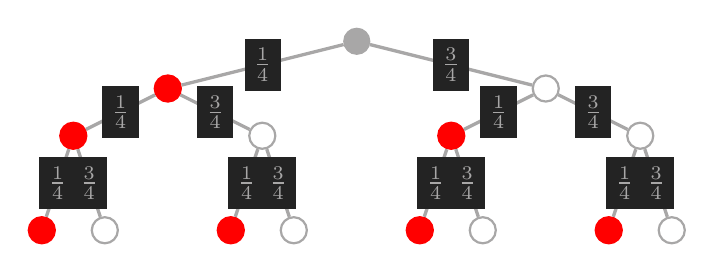
\begin{tikzpicture}[pfeil,yscale=-0.75,scale=0.8] %K weiß, Z rot
	\node[draw,fill,circle] (S) at (0,0) {};
	\node[draw,circle, thick] (K1) at (3,1) {};
	\node[draw,circle, thick, red, fill] (Z1) at (-3,1) {};
	\draw[very thick] (S) -- node[fill=white] {$\frac 34$} (K1);
	\draw[very thick] (S) -- node[fill=white] {$\frac 14$} (Z1);
	\node[draw,circle, thick] (K21) at (4.5,2) {};
	\node[draw,circle, thick, red, fill] (Z21) at (1.5,2) {};
	\draw[very thick] (K1) -- node[fill=white] {$\frac 34$} (K21);
	\draw[very thick] (K1) -- node[fill=white] {$\frac 14$} (Z21);
	\node[draw,circle, thick] (K22) at (-1.5,2) {};
	\node[draw,circle, thick, red, fill] (Z22) at (-4.5,2) {};
	\draw[very thick] (Z1) -- node[fill=white] {$\frac 34$} (K22);
	\draw[very thick] (Z1) -- node[fill=white] {$\frac 14$} (Z22);
	\node[draw,circle, thick] (K31) at (5,4) {};
	\node[draw,circle, thick, red, fill] (Z31) at (4,4) {};
	\draw[very thick] (K21) -- node[fill=white] {$\frac 34$} (K31);
	\draw[very thick] (K21) -- node[fill=white] {$\frac 14$} (Z31);
	\node[draw,circle, thick] (K32) at (2,4) {};
	\node[draw,circle, thick, red, fill] (Z32) at (1,4) {};
	\draw[very thick] (Z21) -- node[fill=white] {$\frac 34$} (K32);
	\draw[very thick] (Z21) -- node[fill=white] {$\frac 14$} (Z32);
	
	\node[draw,circle, thick] (K33) at (-1,4) {};
	\node[draw,circle, thick, red, fill] (Z33) at (-2,4) {};
	\draw[very thick] (K22) -- node[fill=white] {$\frac 34$} (K33);
	\draw[very thick] (K22) -- node[fill=white] {$\frac 14$} (Z33);
	\node[draw,circle, thick] (K34) at (-4,4) {};
	\node[draw,circle, thick, red, fill] (Z34) at (-5,4) {};
	\draw[very thick] (Z22) -- node[fill=white] {$\frac 34$} (K34);
	\draw[very thick] (Z22) -- node[fill=white] {$\frac 14$} (Z34);
\end{tikzpicture}




\end{document}
